\chapter{Tlsfuzzer}
\section{Descrizione}
Tlsfuzzer è un tool per testare implementazioni SSL e TLS. Consente di testare la conformità degli standard di una determinata implementazione, verificare la presenza di vulnerabilità e il fuzzing di connessioni SSL e TLS. Oltre a verificare come il server si comporta di fronte ai test, verifica anche che i massaggi che esso ritorna, anche eventualmente d’errore, siano corretti. Diversamente dal tool TLS-Attacker, con il quale è possibile anche effettuare fuzzing tramite manipolazione dei protocolli di flusso, come descritto nel \textbf{capitolo 1}, il tool tlsfuzzer implementa funzionalità proprie per eseguire l'analisi di vulnerabilità tramite fuzzing. Siccome gli script inclusi in tlsfuzzer si aspettano un comportamento molto specifico dal server, non tutti i risultati negativi dei test e gli errori segnalati dallo script significano necessariamente che il server sia difettoso. $\\$
Tutti gli script di tlsfuzzer presentato il medesimo tipo di output, dove vengono elencati il numero dei test saltati, superati e falliti:$\\$
- VERSION è il numero di versione dello script. Ogni volta che lo script viene modificato in modo tale che la sua esecuzione possa cambiare, la versione viene incrementata.
$\\$
- TOTAL è il numero di connessioni con il server eseguiti dallo script. Ciò però non conteggia solamente il numero di nuove connessioni al server, bensì anche i casi in cui lo script stia testando la ripresa della sessione.
$\\$
-SKIP è il numero di connessioni che sono state escluse dall'esecuzione attraverso l'uso del comando -e.
$\\$
-PASS è il numero di connessioni nelle quali il server si è comportato nel modo previsto (la connessione è andata a buon fine sia quando ci si aspettava un successo, sia quando il server ha rilevato correttamente un messaggio errato quando ne abbiamo inviato uno appositamente).
$\\$
-XFAIL è il numero di connessioni che hanno presumibilmente fallito. Ovvero, il numero di conversazioni specificate con il comando -x e successivamente fallite (senza il messaggio di errore specifico o con il messaggio di errore esatto specificato con il comando -X).
$\\$
-FAIL è il numero di connessioni in cui il server si è comportato in modo inaspettato (ha rifiutato la connessione quando ci si aspettava un successo oppure non ha ritornato un errore quando sono stati inviati messaggi errati)
$\\$
-XPASS è il numero di connessioni che hanno avuto successo in modo inaspettato. Ovvero, le connessioni specificate con il comando -x ma che non hanno fallito.
$\\$
\FloatBarrier
\begin{figure}[h]
    \centering
    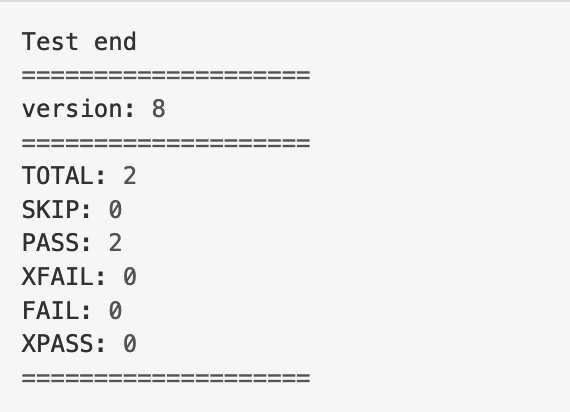
\includegraphics[width = 0.6\textwidth]{images/risultati-tipo-tlsfuzzer.png}
    \caption{Output dello script di test in tlsfuzzer.}
    \label{fig:enter-label}
\end{figure}
\FloatBarrier $\\$

\section{Struttura del tool e creazione di test}
Tlsfuzzer è un tool basato su Python, differentemente da TLS-Attacker analizzato nel capitolo precedente, il quale è costruito su Java. Esso si basa su numerosi script di diverso tipo in Python e presenti nella cartella \textbf{script}. Tuttavia, è possibile creare autonomamente script per poter avere test personalizzati.$\\$
Vediamo quindi come creare un test in modo semplificato. La creazione completa infatti richiede molto codice il quale è disponibile nella pagina github del tool. Per lo scambio di messaggi TLS, gli script necessitano di stabilire dapprima una connessione TCP. E' possibile farlo tramite il seguente codice: $\\$
\begin{verbatim}
    from tlsfuzzer.messages import Connect
     root_node = Connect("localhost", 4433)
     node = root_node
\end{verbatim}$\\$
Il prossimo step consiste nell'inviare un messaggio \textit{ClientHello} al server, contenente la lista delle suite di cifratura:$\\$
\begin{verbatim}
    from tlslite.constants import CipherSuite
    ciphers = [
     CipherSuite.TLS_ECDHE_ECDSA_WITH_AES_128_GCM_SHA256,
     CipherSuite.TLS_ECDHE_RSA_WITH_AES_128_GCM_SHA256,
     CipherSuite.TLS_ECDHE_ECDSA_WITH_AES_128_CBC_SHA,
     CipherSuite.TLS_ECDHE_RSA_WITH_AES_128_CBC_SHA
     ]
\end{verbatim}$\\$
Il server, a sua volta, dovrà rispondere con un \textit{ServerHello}, utilizzando i parametri contenuti nel messaggio inviato dal client:$\\$
\begin{verbatim}
from tlsfuzzer.expect import (
    ExpectServerHello, ExpectCertificate, ExpectServerKeyExchange,
    ExpectServerHelloDone
)
 node = node.add_child(ExpectServerHello())
 node = node.add_child(ExpectCertificate())
 node = node.add_child(ExpectServerKeyExchange())
 node = node.add_child(ExpectServerHelloDone())
\end{verbatim}$\\$
Il client potrà quindi ora generare la propria key e condividerla con il server, il quale, confermandola, chiuderà la procedura di Handshake. 


\section{Utilizzo}
Tlsfuzzer necessita di python per essere utilizzato, in particolare Python2 oppure Python3. Le analisi di vulnerabilità tramite fuzzing possono essere effettuate verso un server aperto localmente, proprio come in TLS-Attacker, oppure verso un qualsiasi altro server esistente. Per aprire un server localmente è possibile usare diverse opzioni, ad esempio \textbf{OpenSSL}. Essa è una libreria software open source ampiamente utilizzata per generare e gestire certificati. Una volta scelto, oppure aperto, un server è possibile iniziare a eseguire diversi script di test, molti dei quali sono già inclusi nel tool. Test verso server comuni come google oppure wikipedia sono abbastanza comuni durante lo studio di questi tipi di tool e non causano danni o rischi alcuni ai server pubblici. Un test che non ritorna casi ‘failed’ si dice che il server è non vulnerabile all’attacco. $\\$
Ad esempio, nella cartella \textit{scrpits} troviamo test-certificate-malformed.py per testare l'invio di un certificato malformato, test-dhe-rsa-key-exchange.py per analizzare il comportamento del server durante lo scambio di chiavi rsa con il client, test-bleichenbacher-workaround.py per effettuare un attacco \textbf{Bleichenbacher- $\\$Workaround}. Quest'ultimo tipo di test è stato eseguito durante la mia analisi del tool, in particolare verso Wikipedia.com. Questo attacco sfrutta delle richieste confezionate ad hoc per ottenere informazioni che consentono di risalire alla chiave utilizzata per crittografare i dati trasmessi tra il server e il browser del visitatore. L'intero codice script del test \textbf{Bleichenbacher-Workaround} è disponibile su Github nella pagina di sviluppo del tool tlsfuzzer. $\\$ $\\$$\\$$\\$
Per eseguire l'attacco la riga di comando da inserire è: $\\$\textit{PYTHONPATH=. python scripts/test-bleichenbacher-workaround.py -h  wikipedia.com -p 443}$\\$
L'opzione \textit{-h} indica il server sul quale esguire l'attacco.$\\$
L'opzione \textit{-p} indica la porta. $\\$
Affinché il test venga eseguito correttamente dobbiamo verificare che possiamo connetterci al server e che possiamo eseguire un handshake, scambiare alcuni dati e chiudere la connessione.
Questo viene fatto dalla parte di codice denominata ‘sanity’ all'interno di ogni script. Se un test fallisce la parte ‘sanity’, non verrà nemmeno effettuato il test vero e proprio. Ad esempio, se vogliamo testare il comportamento di un server alla ricezione di un messaggio ClientHello non corretto, ma dapprima il test ‘sanity’ fallisce (ad esempio fallisce l’handshake), allora lo script non eseguirà proprio il test ClientHello. $\\$
Il test \textbf{Bleichenbacher-Workaround} effettuato verso \textit{wikipedia.com} ha riportato 2 test fail: $\\$
\FloatBarrier
\begin{figure}[h]
    \centering
    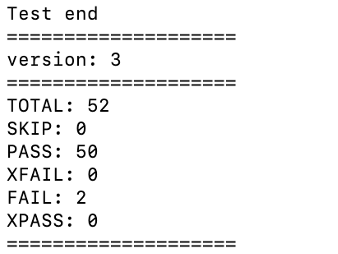
\includegraphics[width = 0.6\textwidth]{images/bleichen-wiki1.png}
    \caption{Output del test Bleichenbacher-Workaround verso Wikipedia.com}
    \label{fig:enter-label}
\end{figure}
\FloatBarrier
$\\$ $\\$$\\$$\\$$\\$
In particolare i 2 test hanno riportato questo errore:$\\$
\FloatBarrier
\begin{figure}[h]
    \centering
    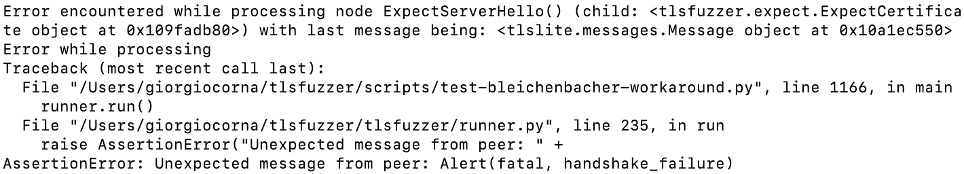
\includegraphics[width = 1.1\textwidth]{images/errore-test-bleichenbacher.png}
    \caption{Errore test Bleichenbacher-Workaround verso Wikipedia.com}
    \label{fig:enter-label}
\end{figure}
\FloatBarrier
$\\$
L’errore riguarda un handshake failure. Ciò significa che il server non ha accettato alcuna crittografia che gli abbiamo inviato. Ciò può accadere quando il server ha solo un certificato ECDSA o non ha abilitato le crittografie necessarie per l'esecuzione del test. Infatti, recandoci sul sito di wikipedia e verificandone tramite il browser il tipo di certificato usato, notiamo che usa proprio un ECDSA. $\\$
\FloatBarrier
\begin{figure}[h]
    \centering
    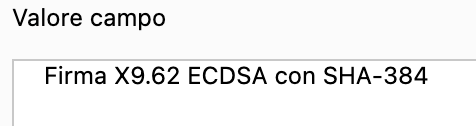
\includegraphics[width = 0.7\textwidth]{images/cert-wiki-ecdsa.png}
    \caption{Certificato utilizzato da Wikipedia.com}
    \label{fig:enter-label}
\end{figure}
\FloatBarrier
$\\$
Tramite il test bleichenbacher-workaround, se il server fallisce solo i ‘sanity’ test, allora la sua configurazione è corretta contro questo attacco. 
$\\$$\\$
Testiamo ora invece uno script su un server aperto in locale con certificato e chiave di tipo RSA. Per prima cosa è necessario, appunto, aprire un server ad hoc per effettuare il test. Creiamo quindi il server con certificato e chiave \textbf{self-signed}. Per definizione, un certificato TLS/SSL autofirmato è un certificato che non è stato firmato da un'autorità di certificazione pubblicamente attendibile, bensì direttamente dallo sviluppatore o dall'azienda che ha aperto il server dove viene utilizzato questo certificato. $\\$
Apertura del server di test: $\\$
\textit{openssl s\_server -key /tmp/localhost.key -cert /tmp/localhost.crt -www} $\\$

$\\$Ora il server è stato aperto correttamente. Eseguo quindi un test per valutare se il server supporta o meno TLS 1.2 o, in alternativa, versioni precedenti con scambio di chiave RSA. Utilizzo lo script \textit{test-conversation.py} presente in tlsfuzzer. $\\$
\FloatBarrier
\begin{figure}[h]
    \centering
    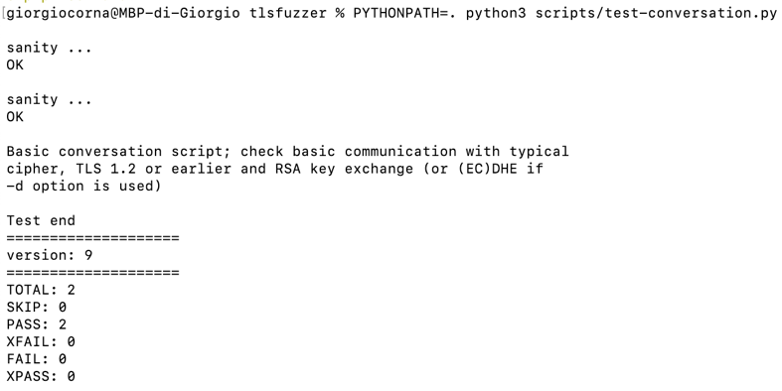
\includegraphics[width = 0.8\textwidth]{images/ris-test-server-local.png}
    \caption{Output del test TLS 1.2 sul server locale}
    \label{fig:enter-label}
\end{figure}
\FloatBarrier
$\\$
Come possiamo notare dai risultati del test, il tool conferma che i test 'sanity' sono stati eseguiti e passati correttamente, per tanto il certificato e la key utilizzate dal server sono conformi al test eseguito. Il server supporta quindi la versione 1.2 del protocollo TLS. $\\$
Riprendendo il server di Wikipedia come esempio, il medesimo test eseguito fallirà, tant'è che Wikipedia non supporta TLS 1.2, in quanto versione datata. Eseguendo invece un test apposito per verificare l'utilizzo da parte del server della più recente versione del protocollo TLS, possiamo notare come questo venga passato correttamente. Notiamo inoltre il nuovo comando utilizzato per eseguire il test \textit{PYTHONPATH=. python scripts/test-tls13-conversation.py -h  wikipedia.com -p 443} diverso dal precedente.  $\\$
\FloatBarrier
\begin{figure}[h]
    \centering
    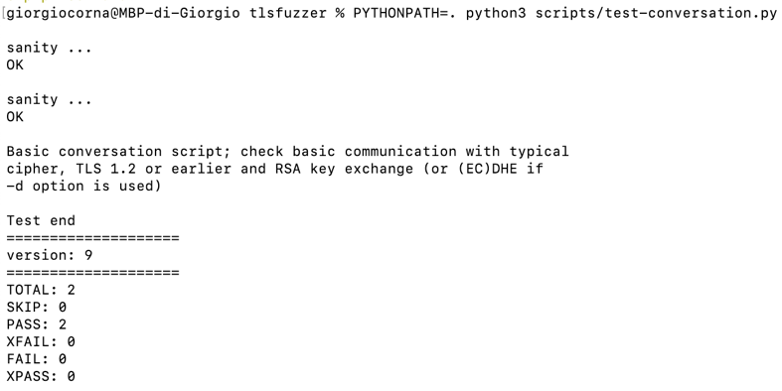
\includegraphics[width = 0.8\textwidth]{images/ris-test-server-local.png}
    \caption{Output del test TLS 1.3 sul server di Wikipedia.com}
    \label{fig:enter-label}
\end{figure}
\FloatBarrier
$\\$

